\section{目的與講義對照}

依講義 PDF 第 94--98 頁，步驟 1 重建圖 24.1 的 8 輸出同步分頻器及圖 24.2 的 4 位元 ripple 計數器，驗證完整分頻週期與操作頻率；步驟 2 比較實際電晶體數、時脈輸入負載及功率。網表 01 包含 7 個週期，02 分離兩電路的時脈電流量測，03 再細化兩個頻率點，共 10 個分析。

\section{電路重建與狀態方程}

所有邏輯由 MOS、靜態閘及 TG latch 組成，不使用理想 DFF 或理想計數器。DFF 使用 22 顆電晶體，reset 同時清除 master 與 slave 狀態，避免解除 reset 時出現非預期計數。同步架構保留圖中的三個 Johnson DFF、兩個三位元同步計數群，以及四 NAND 加一反相器的時脈同步閘；ripple 架構以本級反相輸出驅動下一級正緣時脈。

圖 24.1 的 Johnson 解碼必須照圖判讀：$J_1^+=\overline{J_2}$、$J_2^+=J_1$、$J_3^+=J_2$，$B_0=J_3\oplus\overline{J_2}$、$B_1=J_3$。因此低兩位輸出序列是 1、0、3、2，並非一般遞增二進位碼。兩個三位元群各以 $B_0B_1$ 與 $B_0B_1[B_{4:2}=7]$ 啟用。這裡驗證的是照圖的狀態方程及除 2 至除 256 行為，不將其誤標為普通二進位遞增器。

\section{模擬設定與判讀}

以提供模型、1.0 V、25°C 為教學基準，並非原講義 2.5 V 製程重現或已認證電壓。一般反相器 Wn/Wp/L = 0.6/1.8/0.25 µm，閘內串接元件尺寸在網表明列，每個外部輸出負載 5 fF；時脈邊緣 20 ps。每案例模擬 275 個來源時脈週期，reset 在 1.5T 解除，於第 10 至 269 週期的 0.7T 時點檢查 260 個完整輸出字。時脈上升開始於 0.25T，故輸出建立期限約為 0.45T。

高／低診斷線為 0.8/0.2 V，所有位元都須符合預期才算該字正確。這是宣告的取樣診斷，不是接收器雜訊容限萃取，也不能排除取樣間毛刺。\texttt{.tran} 列印間隔為 T/200；積分步長由求解器自適應。各案例皆完成且沒有 error 或 failed measurement，但加密模型警告內容仍被隱藏。公開網表以 \texttt{MODEL\_SETUP\_REQUIRED} 註解取代載入路徑，執行前需本機模型設定。

\section{波形與傳播時間}

50 MHz 基準中，兩架構皆有 260/260 個完整字符合各自狀態方程。這涵蓋同步架構完整的 256 狀態分頻循環；ripple 輸出則依序遞增，最高位除 16。同步圖低位與高位使用不同時間窗，避免把密集低位切換誤看成穩態。

\begin{figure}[htbp]\centering
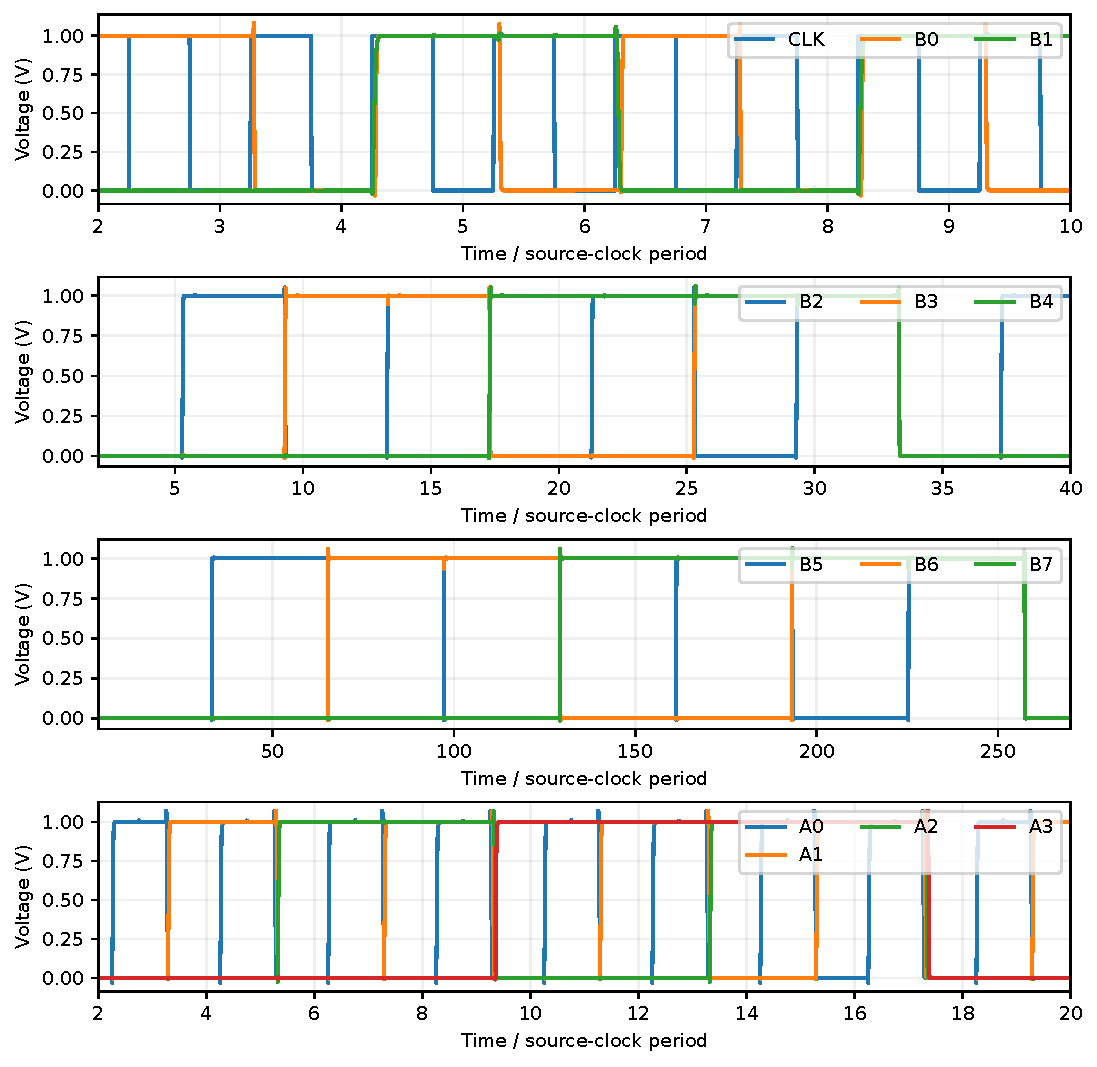
\includegraphics[width=.94\linewidth]{figures/division_waveforms.pdf}
\caption{基準分頻波形；各子圖時間窗不同。}
\end{figure}

ripple 的 7→8 轉換由前級逐級觸發，A0、A1、A2、A3 的半供應交越約落在來源時脈邊緣後 0.532、1.182、1.816、2.263 ns。同步的 B2/B3/B4 群在所選共同轉換中約為 1.012 ns，沒有相同的逐位累積延遲。這些值由 T/200 列印資料線性內插，精度受 100 ps 基準取樣間隔限制；不宣稱 ps 等級簽核精度。

\begin{figure}[htbp]\centering
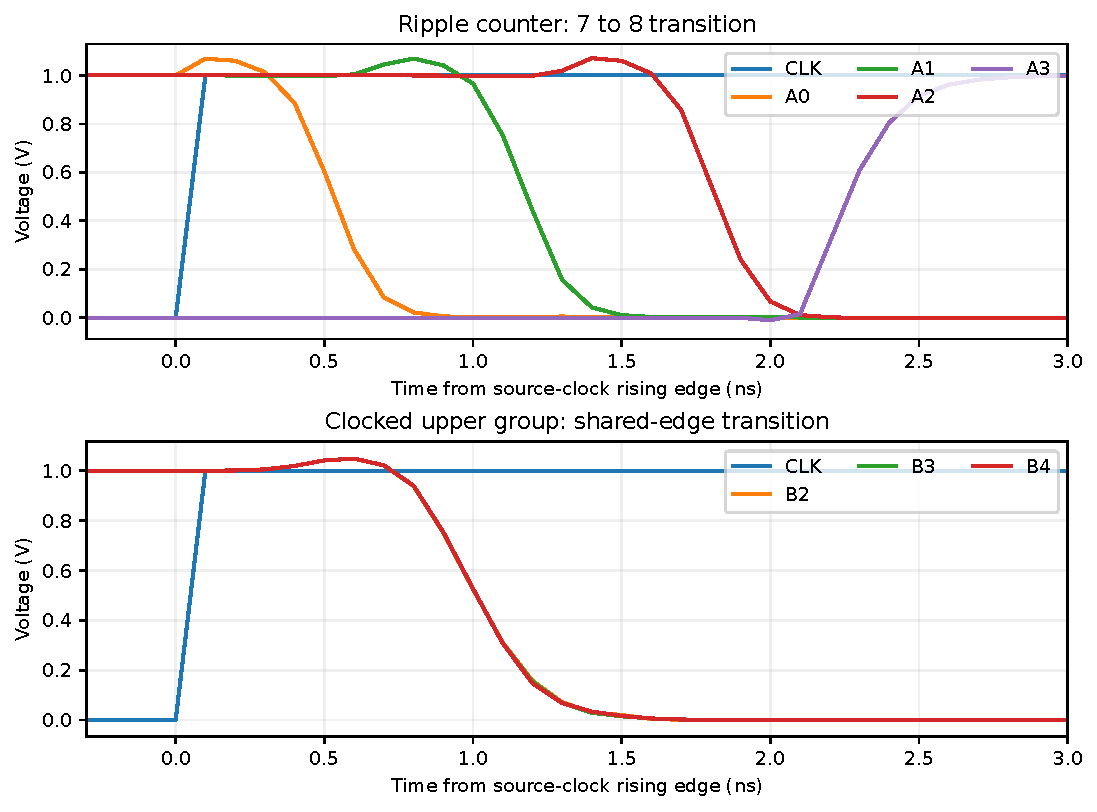
\includegraphics[width=.94\linewidth]{figures/transition_alignment.pdf}
\caption{ripple 累積延遲與同步群的共同轉換。}
\end{figure}

\section{頻率界線與功耗}

\begin{center}\small
\begin{tabular}{lrrr}
\toprule
T (ns) & f (MHz) & 同步正確/260 & Ripple 正確/260 \\
\midrule
20 & 50.0 & 260 & 260 \\
10 & 100.0 & 260 & 260 \\
6 & 166.7 & 260 & 260 \\
5 & 200.0 & 260 & 228 \\
3 & 333.3 & 260 & 195 \\
2.5 & 400.0 & 130 & 130 \\
2 & 500.0 & 130 & 130 \\
1.5 & 666.7 & 0 & 97 \\
1 & 1000.0 & 0 & 0 \\
\bottomrule
\end{tabular}
\end{center}

最高已測且 260/260 正確的同步／ripple 頻率分別為 333.3/166.7 MHz；其上方首個已測失敗點分別為 400.0/200.0 MHz。這是固定負載、20 ps 邊緣與 0.45T 建立期限下的有限掃描界線，不是所有 PVT 的無條件最高頻率。

\begin{figure}[htbp]\centering
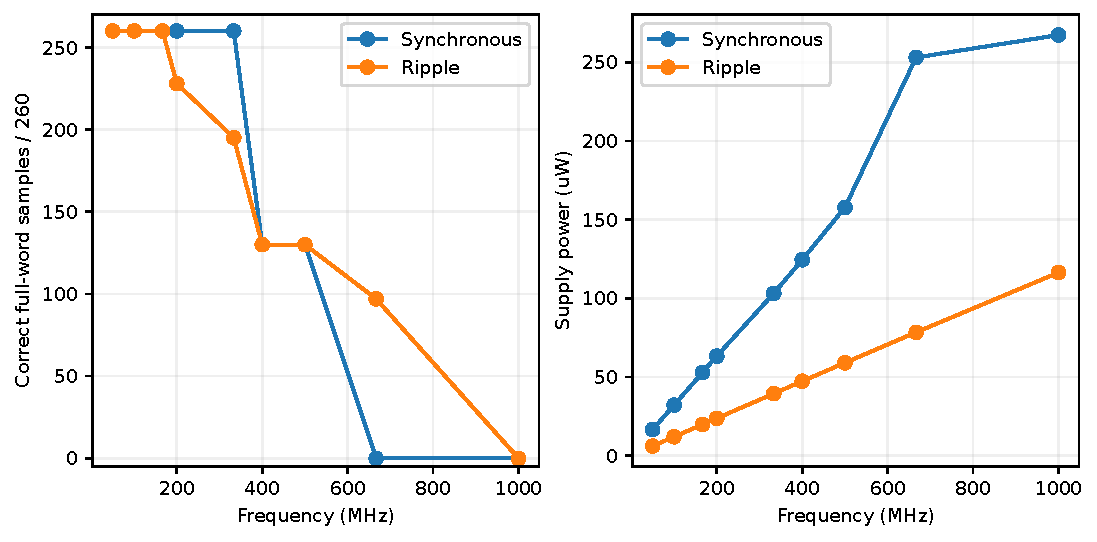
\includegraphics[width=.94\linewidth]{figures/frequency_and_power.pdf}
\caption{取樣正確率與電源功率；失敗頻率的功率仍保留，不能當作正常工作效率。}
\end{figure}

\begin{center}\small
\begin{tabular}{lrrr}
\toprule
架構 & 電晶體 & 時脈邊緣電荷 (fC) & 50 MHz 功率 (µW) \\
\midrule
同步（8 輸出） & 414 & 60.450 & 16.508 \\
Ripple（4 位元） & 98 & 13.474 & 6.034 \\
\bottomrule
\end{tabular}
\end{center}

電晶體數由實際階層網表遞迴計數，包括 clock inverter、同步閘、reset 與 XOR/AND 邏輯，排除未實例化的副電路。時脈負載由第 10.25T 上升邊緣期間獨立 0 V 探針電流積分量測；1 V 擺幅下 Q/ΔV 對應約 60.450/13.474 fF 的此邊緣等效負載，並非版圖電容。功率為 10T--270T 的平均供應功率，未計入理想時脈及 reset 驅動源的功率。

\section{討論與限制}

同步架構以更多時脈負載與邏輯換取較小的逐級延遲；ripple 則減少直接時脈負載，但必須等待前級切換。本講義比較 8 輸出與 4 位元兩種不同規模，故不能把總功率差當作相同功能、相同位數的公平效率比。沒有強迫結果符合講義 1 GHz/500 MHz 的原製程範例，也沒有用理想計數器掩蓋最高頻率失敗。所有逐案例波形、完整字判讀及量測保留於 results。
